\begin{tikzpicture}[scale=0.52]
	\begin{axis} [
		title = {\LARGE $\barc\opH_\degp(X)$, if $\opH_\degp(X_0) \neq 0$},
		ticklabel style = {font=\Large},
		axis y line=middle,
		axis x line=middle,
		ytick={0.7,0.76,0.8,0.95},
		yticklabels={$\beta_\degp$,,,$R$},
		xtick={0.55,0.95},
		xticklabels={$\alpha$, $R$},
		xmin=-0.015, xmax=1.1,
		ymin=0, ymax=1.1,]
		\addplot [mark=none] coordinates {(0,0) (1,1)};
		\addplot [thick,color=black!20!white,fill=black!30!white,
		fill opacity=0.4]coordinates {
			(0.55,0.95)
			(0.55,0.55)
			(0.95,0.95)
			(0.55,0.95)};
		\addplot [black!40!white,mark=none,dashed, thin] coordinates {(0,0.7) (0.7,0.7)};
		\addplot [black!40!white,mark=none,dashed, thin] coordinates {(0,0.55) (0.55,0.55)};
		\addplot [black!40!white,mark=none,dashed, thin] coordinates {(0.55,0) (0.55,0.55)};
		\addplot[barccolor,mark=*] (0, 0.7) circle (2pt) node[above right,barccolor]{};
            \addplot[barccolor,mark=*] (0, 0.76) circle (2pt) node[above right,barccolor]{};
            \addplot[barccolor,mark=*] (0, 0.8) circle (2pt) node[above right,barccolor]{};
		%\node[mark=none] at (axis cs:0.68,0.21){$\Hbarc{2}{\VS^n}$};
	\end{axis}
\end{tikzpicture}
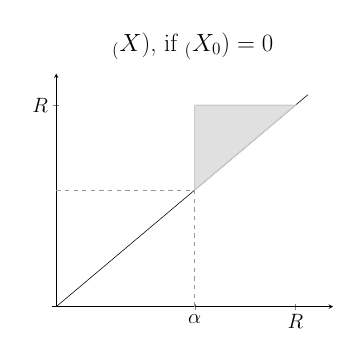
\begin{tikzpicture}[scale=0.52]
	\begin{axis} [
		title = {\LARGE $\barc\opH_\degp(X)$, if $\opH_\degp(X_0) = 0$},
		ticklabel style = {font=\Large},
		axis y line=middle,
		axis x line=middle,
		ytick={0.95},
		yticklabels={$R$},
		xtick={0.55,0.95},
		xticklabels={$\alpha$, $R$},
		xmin=-0.015, xmax=1.1,
		ymin=0, ymax=1.1,]
		\addplot [mark=none] coordinates {(0,0) (1,1)};
		\addplot [thick,color=black!20!white,fill=black!30!white,
		fill opacity=0.4]coordinates {
			(0.55,0.95)
			(0.55,0.55)
			(0.95,0.95)
			(0.55,0.95)};
		\addplot [black!40!white,mark=none,dashed, thin] coordinates {(0,0.55) (0.55,0.55)};
		\addplot [black!40!white,mark=none,dashed, thin] coordinates {(0.55,0) (0.55,0.55)};
	\end{axis}
\end{tikzpicture}

\begin{tikzpicture}[scale=0.52]
	\begin{axis} [
		title={\LARGE $\barc\img\theta_{X}$, if $\img\theta_{X_0}\neq 0$},
		ticklabel style = {font=\Large},
		axis y line=middle,
		axis x line=middle,
		ytick={0.7,0.74,0.82,0.95},
		yticklabels={$\gamma_\degp$,,,$R$},
		xtick={0.55,0.95},
		xticklabels={$\alpha$, $R$},
		xmin=-0.015, xmax=1.1,
		ymin=0, ymax=1.1,]
		\addplot [mark=none] coordinates {(0,0) (1,1)};
		\addplot [thick,color=black!20!white,fill=black!30!white,
		fill opacity=0.4]coordinates {
			(0.55,0.95)
			(0.55,0.55)
			(0.95,0.95)
			(0.55,0.95)};
		\addplot [black!40!white,mark=none,dashed, thin] coordinates {(0,0.7) (0.7,0.7)};
		\addplot [black!40!white,mark=none,dashed, thin] coordinates {(0,0.55) (0.55,0.55)};
		\addplot [black!40!white,mark=none,dashed, thin] coordinates {(0.55,0) (0.55,0.55)};
		\addplot[barccolor,mark=*] (0, 0.7) circle (2pt) node[above right,barccolor]{};
            \addplot[barccolor,mark=*] (0, 0.74) circle (2pt) node[above right,barccolor]{};
            \addplot[barccolor,mark=*] (0, 0.82) circle (2pt) node[above right,barccolor]{};
		%\node[mark=none] at (axis cs:0.68,0.21){$\Hbarc{2}{\VS^n}$};
	\end{axis}
\end{tikzpicture}
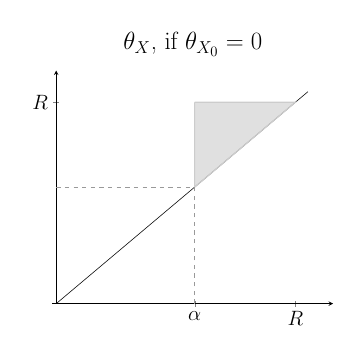
\begin{tikzpicture}[scale=0.52]
	\begin{axis} [
		title={\LARGE $\barc\img\theta_{X}$, if $\img\theta_{X_0}= 0$},
		ticklabel style = {font=\Large},
		axis y line=middle,
		axis x line=middle,
		ytick={0.95},
		yticklabels={$R$},
		xtick={0.55,0.95},
		xticklabels={$\alpha$, $R$},
		xmin=-0.015, xmax=1.1,
		ymin=0, ymax=1.1,]
		\addplot [mark=none] coordinates {(0,0) (1,1)};
		\addplot [thick,color=black!20!white,fill=black!30!white,
		fill opacity=0.4]coordinates {
			(0.55,0.95)
			(0.55,0.55)
			(0.95,0.95)
			(0.55,0.95)};
		\addplot [black!40!white,mark=none,dashed, thin] coordinates {(0,0.55) (0.55,0.55)};
		\addplot [black!40!white,mark=none,dashed, thin] coordinates {(0.55,0) (0.55,0.55)};
	\end{axis}
\end{tikzpicture}